%%%%%%%%%%%%%%%%%%%%%%%%%%%%%%%%%%%%%%%%%%%%%%%%%%%%%%%%%%%%%%%%%%%
%                                                                 %                    
%                 Packages / Grundeinstellungen                   %
%                                                                 %
%%%%%%%%%%%%%%%%%%%%%%%%%%%%%%%%%%%%%%%%%%%%%%%%%%%%%%%%%%%%%%%%%%%
\DocumentMetadata{
    pdfversion=2.0,
    pdfstandard=A-4,
}

\documentclass[paper=a1,parskip=half,fontsize=24]{scrartcl}

\usepackage[ngerman]{babel}
\usepackage{lmodern}
\usepackage{fontspec}
\usepackage{calc}
\usepackage{microtype}
\usepackage{tcolorbox}
\usepackage{blindtext}
\usepackage{float}
\usepackage{subcaption}

% Keine floats in andere Sections
\usepackage[section]{placeins}

% Eurozeichen einbinden
\usepackage[right]{eurosym}

% Floatende Bilder ermöglichen
\usepackage{floatflt}

% Bricht lange URLs "schön" um
\usepackage[hyphens,obeyspaces,spaces]{url}

% Mathematische Symbole importieren
\usepackage{amssymb}

% Zitierung nach APA
%\usepackage[
%backend=biber,
%style=apa,
%autocite=inline,
%]{biblatex}
%\addbibresource{bibtex/poster.bib}

% Zitierung nach IEEE
\usepackage[
backend=biber,
style=ieee,
autocite=inline,
]{biblatex}
\addbibresource{bibtex/poster.bib}

\setcounter{biburllcpenalty}{7000}
\setcounter{biburlucpenalty}{8000}

% Paket für Zeilenabstand
\usepackage{setspace}

% Für Bildbezeichner
\usepackage{capt-of}

% Für Stichwortverzeichnis
\usepackage{makeidx}

% Erzeugt Inhaltsverzeichnis mit Querverweisen zu den Abschnitten (PDF Version)
\usepackage[bookmarksnumbered,hyperfootnotes=false,hypertexnames=false]{hyperref}
\hypersetup{
  colorlinks=true,
  linkcolor=black,
  filecolor=blue,
  citecolor = black,      
  urlcolor=blue,
  }

%mehrspaltig
\usepackage{multicol} 
\columnsep=70pt 
\columnseprule=3pt 

%grafiken einbinden
\usepackage{graphicx}

% Booktabs Tabellen
\usepackage{tabularray}
\UseTblrLibrary{booktabs}
\DefTblrTemplate{contfoot-text}{normal}{Fortsetzung auf nächster Seite}
\SetTblrTemplate{contfoot-text}{normal}
\DefTblrTemplate{conthead-text}{normal}{}
\SetTblrTemplate{conthead-text}{normal}

% Paket für Textfarben
\usepackage{xcolor} 
\definecolor{LightGray}{gray}{0.9}
\usepackage[pagecolor=white]{pagecolor}

% Für schönere Listings
\usepackage[outputdir=log, newfloat,]{minted}
\setminted{
  frame=lines,
  framesep=2mm,
  baselinestretch=1.2,
  bgcolor=LightGray,
  fontsize=\footnotesize,
  linenos,
  breaklines=true,
  breakanywhere=true,
  autogobble,
  tabsize=2
}
\setmintedinline{}

% Keine Floats bei Listings
\newenvironment{code}[2]
  {
  \providecommand{\captiontitle}{#1}
  \providecommand{\labeltitle}{#2}
  \vspace*{0.3cm}
  }
  {
  %\vspace*{-2.0cm}
  \captionbelowof{listing}{\captiontitle}
  \label{\labeltitle}
  \vspace*{0.35cm}
  }
\SetupFloatingEnvironment{listing}{}

%seitengeometrie
\usepackage{geometry}
\geometry{margin=3cm,top=3cm}

%Definition Schrift- und Farbeinstellungen 
\setmainfont{TeX Gyre Termes}
\setsansfont{TeX Gyre Adventor}
\usepackage{preamble}


%Siehe hierzu preamble.sty
\colorlet{basecolor}{meerblau}
\colorlet{akzentcolor}{mint}

%Siehe hierzu preamble.sty
%\renewcommand{\theauthor}{Thore Hüneke thohueneke, Anette Michlik anemichlik, Kasem Rashrash kasrashrash, Sophie Sergeenko sopsergeenko}
%\renewcommand{\thetitle}{Impftermine digital: Schnell. Sicher. Skalierbar.}
%\renewcommand{\thesubtitle}{Von der Idee zur technischen Umsetzung}

%Höhe des HS Logos 4cm für zweizeiligen Titel, 2.5cm für einzeiligen Titel
\newcommand{\myspace}{4cm}

\hypersetup{pdfinfo={
  Title={\thetitle},
  Author={\theauthor}
}}

% Darf erst hier eingebunden werden! 
\usepackage{csquotes}

%Textfarbe
\color{black}

%%%%%%%%%%%%%%%%%%%%%%%%%%%%%%%%%%%%%%%%%%%%%%%%%%%%%%%%%%%%%%%%%%%
%                                                                 %                    
%                     Beginn des Inhalts                          %
%                                                                 %
%%%%%%%%%%%%%%%%%%%%%%%%%%%%%%%%%%%%%%%%%%%%%%%%%%%%%%%%%%%%%%%%%%%

%%%%%%%%%%%%%%%%%%%%%%%%%%%%%%%%%%%%%%%%%%%%%%%%%%%%%%%%%%%%%%%%%%%
%  Special Characters:                                            %
%                                                                 %
%             \& \% \$ \# \_ \{ \}                                %
%             \textasciitilde (~)                                 %
%             \textasciicircum (^)                                %     
%             \textbackslash (\)                                  %                    
%      \glqq Text\grqq{} für Anführungszeichen                    %
%%%%%%%%%%%%%%%%%%%%%%%%%%%%%%%%%%%%%%%%%%%%%%%%%%%%%%%%%%%%%%%%%%%


\begin{document}
  %Printed Überschriften
  %\thetitlearea
  %Mehrspaltig
  \begin{multicols*}{3}
  
    % Input Inhalt
    \section*{Architekturmodellierung}
Ein funktionierendes System benötigt eine klare Architektur, die sicherstellt, dass Daten 
effizient verarbeitet, gespeichert und bereitgestellt werden.
Die Impfregistrierungsanwendung besteht aus mehreren technischen Komponenten, die 
zusammenarbeiten und einer Client-Server-Architektur folgen, bei der das
Frontend, Backend und die Datenbank klar voneinander getrennt sind.
Die Architekturmodellierung der Anwendung begann mit der Entwicklung eines Fachmodells, 
das die zentralen Entitäten und deren Beziehungen beschreibt. Dieses Modell diente als 
Grundlage für die funktionale Struktur der Anwendung und ermöglichte eine klare 
Definition der Geschäftslogik.

\begin{center}
  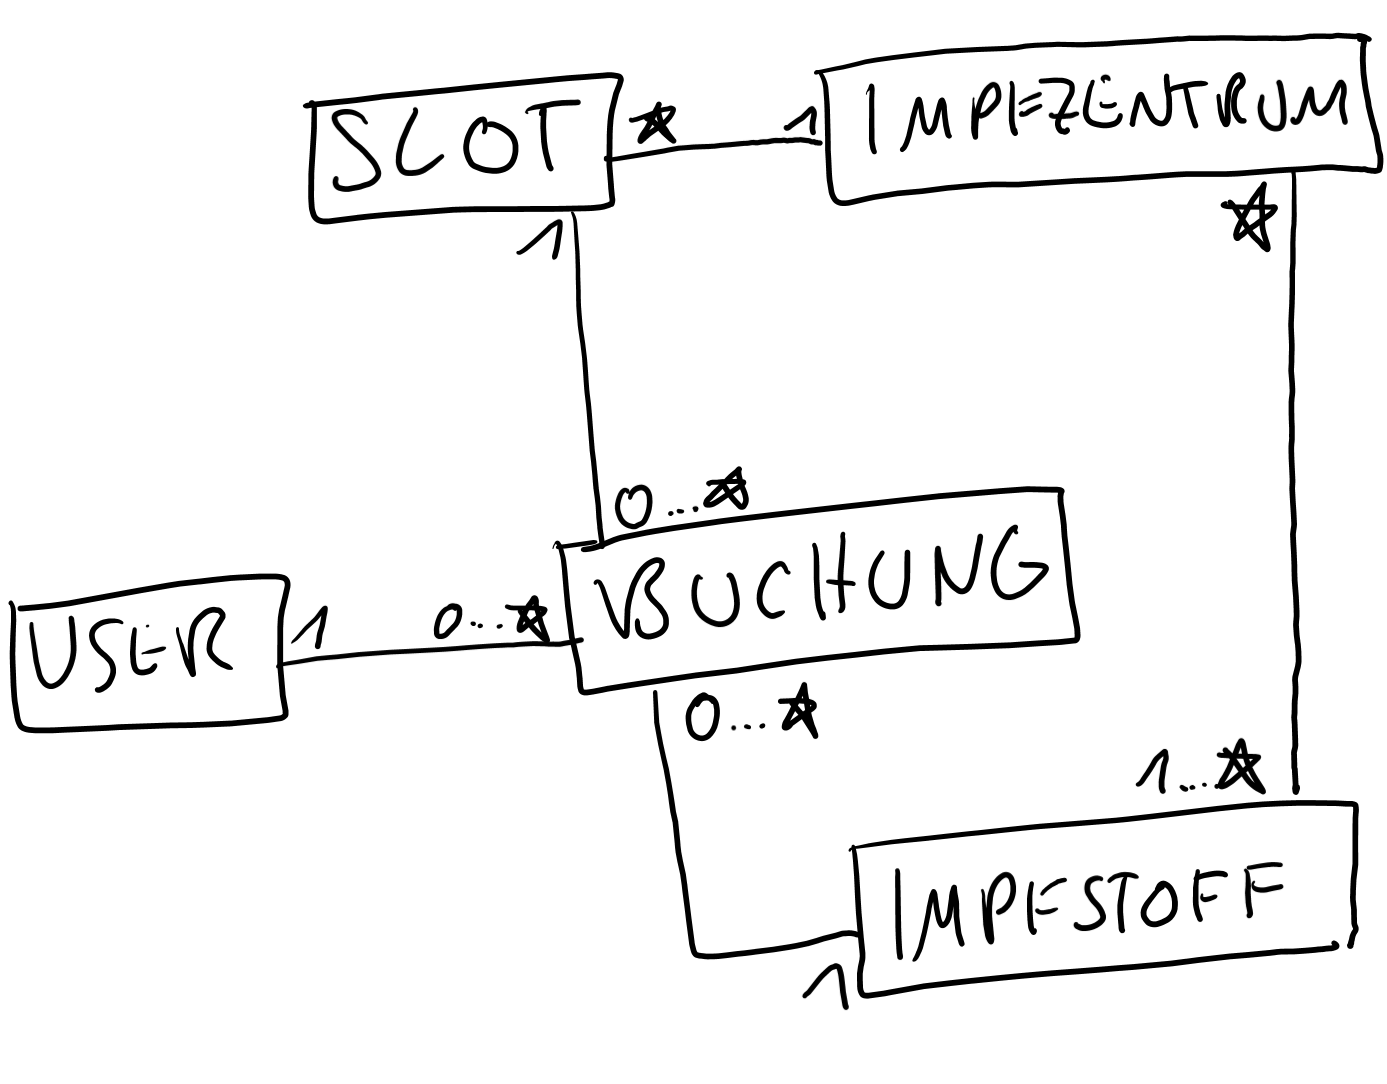
\includegraphics[width=0.95\linewidth, height=0.45\textheight, keepaspectratio]{src/abbildungen/fachmodell.PNG}
  \captionof{figure}{Fachmodell}
\end{center}

Basierend auf dem Fachmodell wurde anschließend ein relationales Datenmodell entwickelt, 
das die Speicherung und Verwaltung der Daten in der Datenbank strukturiert. 

\begin{center}
  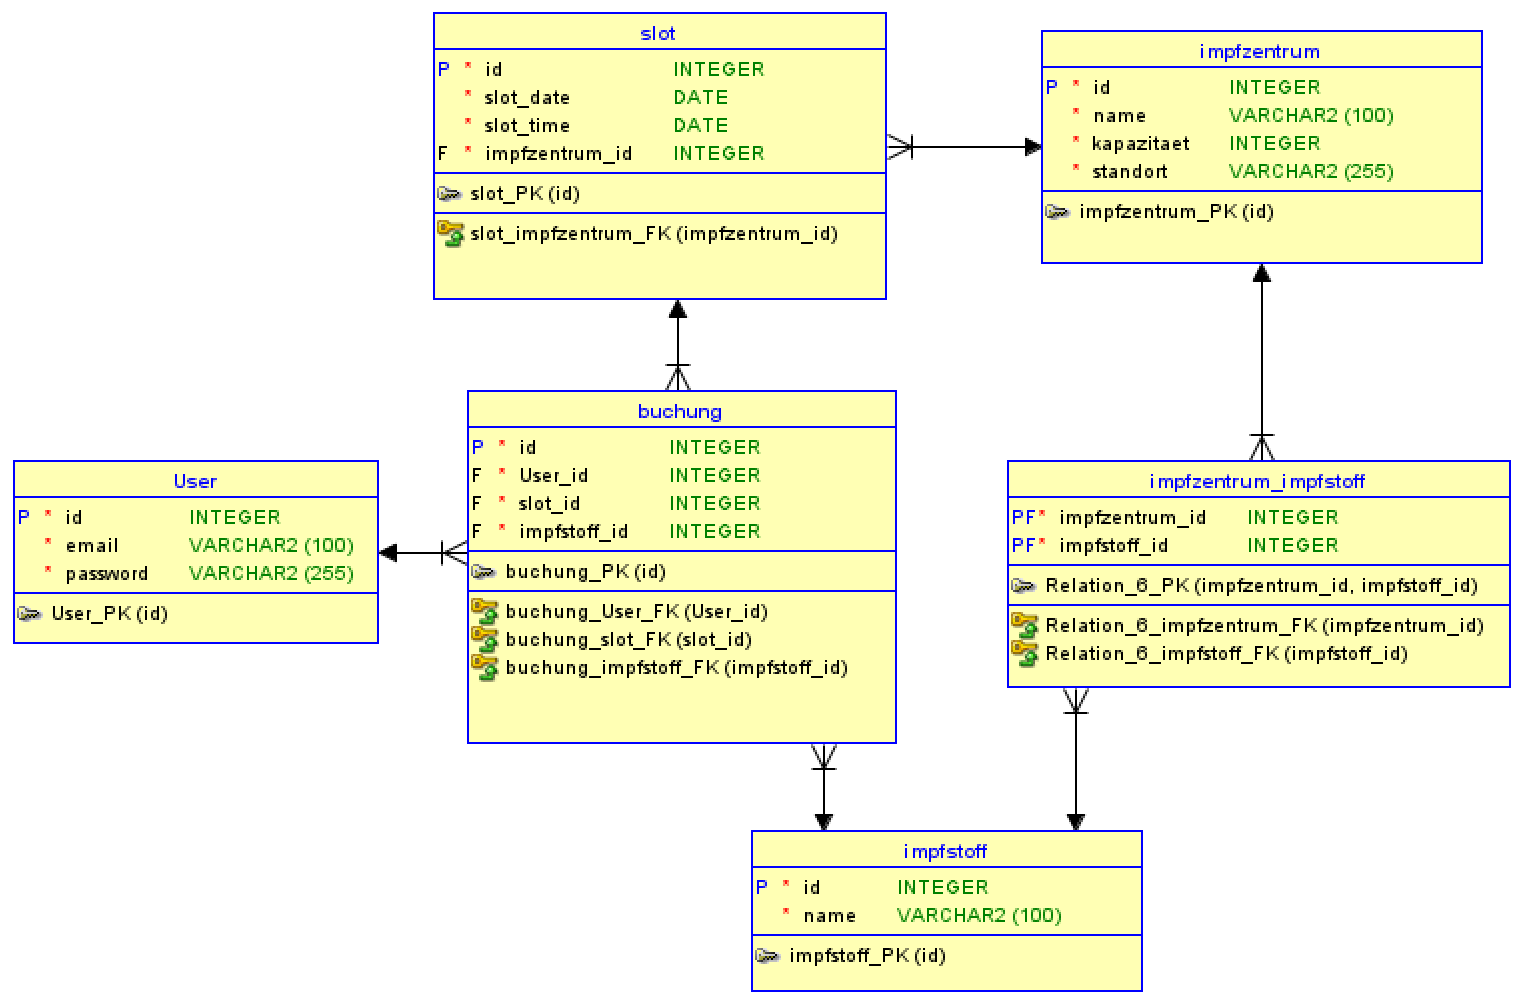
\includegraphics[width=0.95\linewidth, height=0.45\textheight, keepaspectratio]{src/abbildungen/relmodell.png}
  \captionof{figure}{Relationales Modell}
\end{center}

    \section*{Anfragenverarbeitung}
Das Backend basiert auf einer Servlet-Architektur, die Anfragen aus dem Frontend 
entgegennimmt, verarbeitet und die entsprechenden Daten zurückliefert. Sobald ein Nutzer 
beispielsweise einen Termin buchen möchte, sendet das Frontend eine HTTP-Anfrage an das 
Backend. Diese wird von einem passenden Servlet empfangen und verarbeitet. Wenn der 
Nutzer weniger als vier Buchungen hat, wird die neue Buchung gespeichert und an das 
Frontend zurückgemeldet.
Die Architektur des Backends ist in mehrere komplementäre Module unterteilt:
\begin{itemize}
    \item Servlets: Nehmen Anfragen aus dem Frontend entgegen, verarbeiten sie und leiten sie an die passenden Komponenten weiter.
    \item Skripte für Datenbankabfragen: Enthalten SQL-Abfragen, um strukturierte Datenbankinteraktionen zu ermöglichen.
    \item Utility-Klassen: Stellen allgemeine Funktionen bereit, die wiederverwendet werden können, wie etwa Passwort-Hashing.
\end{itemize}
Durch diese klare Trennung der Verantwortlichkeiten bleibt der Code modular und gut 
wartbar. Änderungen an einzelnen Komponenten beeinflussen nicht das gesamte System, 
wodurch die Stabilität und Skalierbarkeit der Anwendung gewährleistet wird. Die klare
Struktur erleichterte zudem die Zusammenarbeit im Team, insbesondere für Mitglieder mit 
unterschiedlichem Erfahrungsniveau. Gegen Ende des Projekts zeigte sich jedoch, dass 
diese Arbeitsweise auch Performance-Nachteile haben kann – mehr dazu auf Poster Drei. 

    \section*{Dynamische Terminbuchung}
Das Frontend wurde als Single Page Anwendung (SPA) geschrieben. Eine SPA ermöglicht es, 
Inhalte dynamisch nachzuladen, ohne dass die gesamte Seite neu geladen werden muss. Dies 
sorgt für eine schnelle und unterbrechungsfreie Benutzererfahrung, da die Anwendung stets 
direkt auf Nutzerinteraktionen reagieren kann.
Ein zentraler Bestandteil des Frontends ist die dynamische Verwaltung von Impfterminen. 
Nutzer können über die Anwendung verfügbare Termine einsehen, Buchungen vornehmen und 
bestehende Reservierungen verwalten. Diese Funktionen werden über verschiedene 
JavaScript-Dateien gesteuert.
Beim Aufruf der Terminbuchungsseite wird automatisch eine asynchrone Anfrage mittels AJAX
an das Backend gestellt, um die aktuell verfügbaren Termine in einem Kalender abzurufen. 
Dadurch werden dem Nutzer nur tatsächlich buchbare Slots angezeigt. Zusätzlich wird 
sichergestellt, dass bereits gebuchte oder abgelaufene Termine nicht mehr auswählbar sind.
%\begin{center}
%  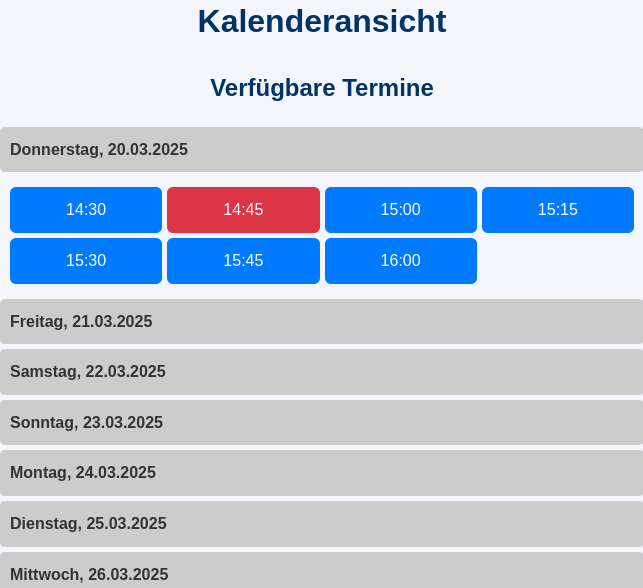
\includegraphics[width=0.95\linewidth, height=0.45\textheight, keepaspectratio]{src/abbildungen/kalenderansicht.png}
%  \captionof{figure}{Kalenderansicht}
%\end{center}
Ein wesentlicher Vorteil dieses Konzepts ist die verbesserte Performance der Anwendung. 
Statt bei jeder Benutzeraktion eine komplette neue Seite zu laden, werden nur die 
tatsächlich benötigten Daten nachgefordert. Dies reduziert nicht nur die Ladezeiten, 
sondern verringert auch die Serverlast, da weniger Daten übertragen werden müssen. 

    \section*{Cronjob für die Kalenderlogik}
Damit das System jederzeit aktuelle Terminverfügbarkeiten anzeigt und alte Daten nicht 
unnötig Speicherplatz belegen, wurde eine automatisierte Kalenderlogik in Form eines 
SQL-Cronjobs implementiert. Diese geplante SQL-Prozedur läuft täglich und übernimmt zwei 
Hauptaufgaben: Das Entfernen abgelaufener Buchungen des Vortags und die automatische 
Generierung neuer Zeitslots für den kommenden Tag.
Durch die Automatisierung entfällt die manuelle Terminaktualisierung, und die Datenbank 
bleibt performant, da veraltete Einträge regelmäßig entfernt werden.
Ein wesentlicher Vorteil dieser Lösung ist ihre Skalierbarkeit. Da die Terminverwaltung 
durch einen zentralen Cronjob erfolgt und die Zeitslots im Voraus generiert werden, 
bleibt das System auch bei hoher Last stabil. Nutzeranfragen greifen lediglich auf die 
bereits vorbereiteten Daten zu, wodurch keine zusätzliche Last entsteht.
Darüber hinaus können neue Impfzentren problemlos hinzugefügt werden, ohne dass 
Anpassungen an der Buchungslogik notwendig sind. Die tägliche Aktualisierung der Termine 
gewährleistet, dass das System stets aktuelle und korrekte Daten liefert, während der 
Wartungsaufwand auf ein Minimum reduziert bleibt.

    \section*{Schutz der Nutzerdaten}
Da das System personenbezogene Informationen wie Nutzerdaten und Buchungsdetails 
verarbeitet, wurden verschiedene Sicherheitsmaßnahmen implementiert, um unbefugten 
Zugriff zu verhindern, die Datenintegrität zu gewährleisten und den 
Datenschutzbestimmungen zu entsprechen.
Eine wichtige Rolle spielt das Session-Handling. Nach einer erfolgreichen Anmeldung 
bleibt der Nutzer über eine Sitzung authentifiziert, sodass er nicht bei jeder Aktion 
erneut seine Zugangsdaten eingeben muss. Um die Sicherheit zu erhöhen, wird die Sitzung 
nach einer Inaktivitätszeit von 2 Minuten automatisch beendet. Dies schützt vor 
Missbrauch durch offene Sitzungen auf unbeaufsichtigten Geräten.
Zusätzlich wird bei einer abgelaufenen Sitzung ein Overlay angezeigt, das den Nutzer zur 
erneuten Anmeldung auffordert. 
\begin{center}
  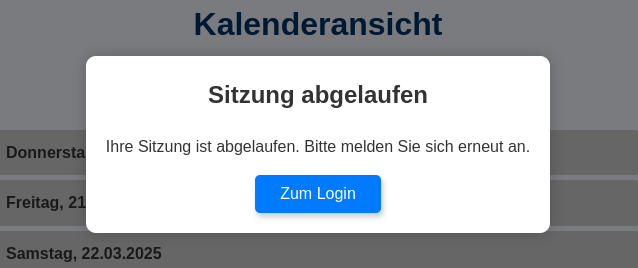
\includegraphics[width=0.95\linewidth, height=0.45\textheight, keepaspectratio]{src/abbildungen/session.png}
  \captionof{figure}{Sitzung abgelaufen}
\end{center}
Die Sitzungsinformationen werden ausschließlich 
serverseitig verwaltet und nicht im Browser gespeichert, um die Gefahr des 
Sitzungsdiebstahls zu minimieren. Um sicherzustellen, dass die Sitzungs-Cookies gegen 
Angriffe geschützt sind, wurden bestimmte Attribute gesetzt.
\vspace{0.5cm}
\begin{lstlisting}[language=java, caption={Cookie-Attribute}, captionpos=b]
 session.setMaxInactiveInterval(120);
 Cookie sessionCookie = new Cookie("JSESSIONID", session.getId());
 sessionCookie.setHttpOnly(true);
 sessionCookie.setSecure(true); 
 sessionCookie.setAttribute("SameSite", "Strict"); 
 response.addCookie(sessionCookie);
\end{lstlisting}
Sollte sich ein Nutzer ausloggen oder eine Sitzung ablaufen, wird die Session sofort 
ungültig gemacht, um Missbrauch durch Dritte zu verhindern.
Ein weiterer Aspekt ist die sichere Speicherung von Passwörtern. Um Nutzerkonten vor 
Brute-Force-Angriffen und kompromittierten Datenbanken zu schützen, werden Passwörter mit 
dem Algorithmus PBKDF2 gehasht. Dieser nutzt eine hohe Anzahl von Iterationen und einen 
zufälligen Salt-Wert, um den Rechenaufwand für Angreifer zu steigern.Dadurch wird 
verhindert, dass vorberechnete Hash-Tabellen (Rainbow Tables) verwendet werden können.
Ebenfalls wichtig zu erwähnen ist die Verwendung von QR-Codes zur Terminverifizierung. 
Nach einer erfolgreichen Terminbuchung erhalten Nutzer eine Buchungsbestätigung per Mail 
als PDF mit einem QR-Code, der bei der Ankunft im Impfzentrum gescannt wird. Um den 
Datenschutz zu gewährleisten, enthält der QR-Code jedoch keine sensiblen Informationen, 
sondern lediglich eine Buchungs-ID, die beim Scannen mit der Datenbank abgeglichen wird. 
Selbst wenn ein QR-Code in falsche Hände gerät, können daraus keine Rückschlüsse auf die 
Identität des Nutzers gezogen werden. Diese Maßnahme entspricht den Bestimmungen der 
DSGVO und stärkt das Vertrauen der Nutzer in die Anwendung.

    
    % Literaturverzeichnis anzeigen
    %\section*{Referenzen}
    %\vspace*{0.3cm}
    %\printbibliography[heading=none]

  \end{multicols*}
\end{document}

